%%\documentclass[a4paper, 12pt]{scrreprt}

\documentclass[a4paper, 12pt]{scrartcl}
%usepackage[german]{babel}
\usepackage{microtype}
%\usepackage{amsmath}
%usepackage{color}
\usepackage[utf8]{inputenc}
\usepackage[T1]{fontenc}
\usepackage{wrapfig}
\usepackage{lipsum}% Dummy-Text
\usepackage{multicol}
\usepackage{alltt}
%%%%%%%%%%%%bis hierhin alle nötigen userpackage
\usepackage{tabularx}
\usepackage[utf8]{inputenc}
\usepackage{amsmath}
\usepackage{amsfonts}
\usepackage{amssymb}
\usepackage{graphicx}
\usepackage{longtable}
\usepackage{booktabs}
\usepackage{tabularx}
\usepackage{siunitx}

%\usepackage{wrapfig}
\usepackage[ngerman]{babel}
\usepackage[left=25mm,top=25mm,right=25mm,bottom=25mm]{geometry}
%\usepackage{floatrow}
\setlength{\parindent}{0em}
\usepackage[font=footnotesize,labelfont=bf]{caption}
\numberwithin{figure}{section}
\numberwithin{table}{section}
\usepackage{subcaption}
\usepackage{float}
\usepackage{url}
\usepackage{fancyhdr}
\usepackage{array}
\usepackage{geometry}
%\usepackage[nottoc,numbib]{tocbibind}
\usepackage[pdfpagelabels=true]{hyperref}
\usepackage[font=footnotesize,labelfont=bf]{caption}
\usepackage[T1]{fontenc}
\usepackage {palatino}
%\usepackage[numbers,super]{natbib}
%\usepackage{textcomp}
\usepackage[version=4]{mhchem}

\usepackage{hyperref}
%\begin{document}

\section{Auswertung}

Es wurde die Veränderung des optischen Drehwinkels $\alpha$ in Relation zu der Zeit bei unterschiedlichen Temperaturen gemessen. Diese Werte wurden in Abbildung \ref{at} dargestellt. Der Winkel nimmt exponentiell mit der Zeit bei allen gewählten Temperaturen ab. Die Messwerte wurden mit der Gleichung 10 angepasst, wodurch $\alpha_0$, $\alpha_\infty$ und $k$ bestimmt werden konnten.


\begin{figure}[h]
	\centering	
	\begin{minipage}{1\textwidth}
	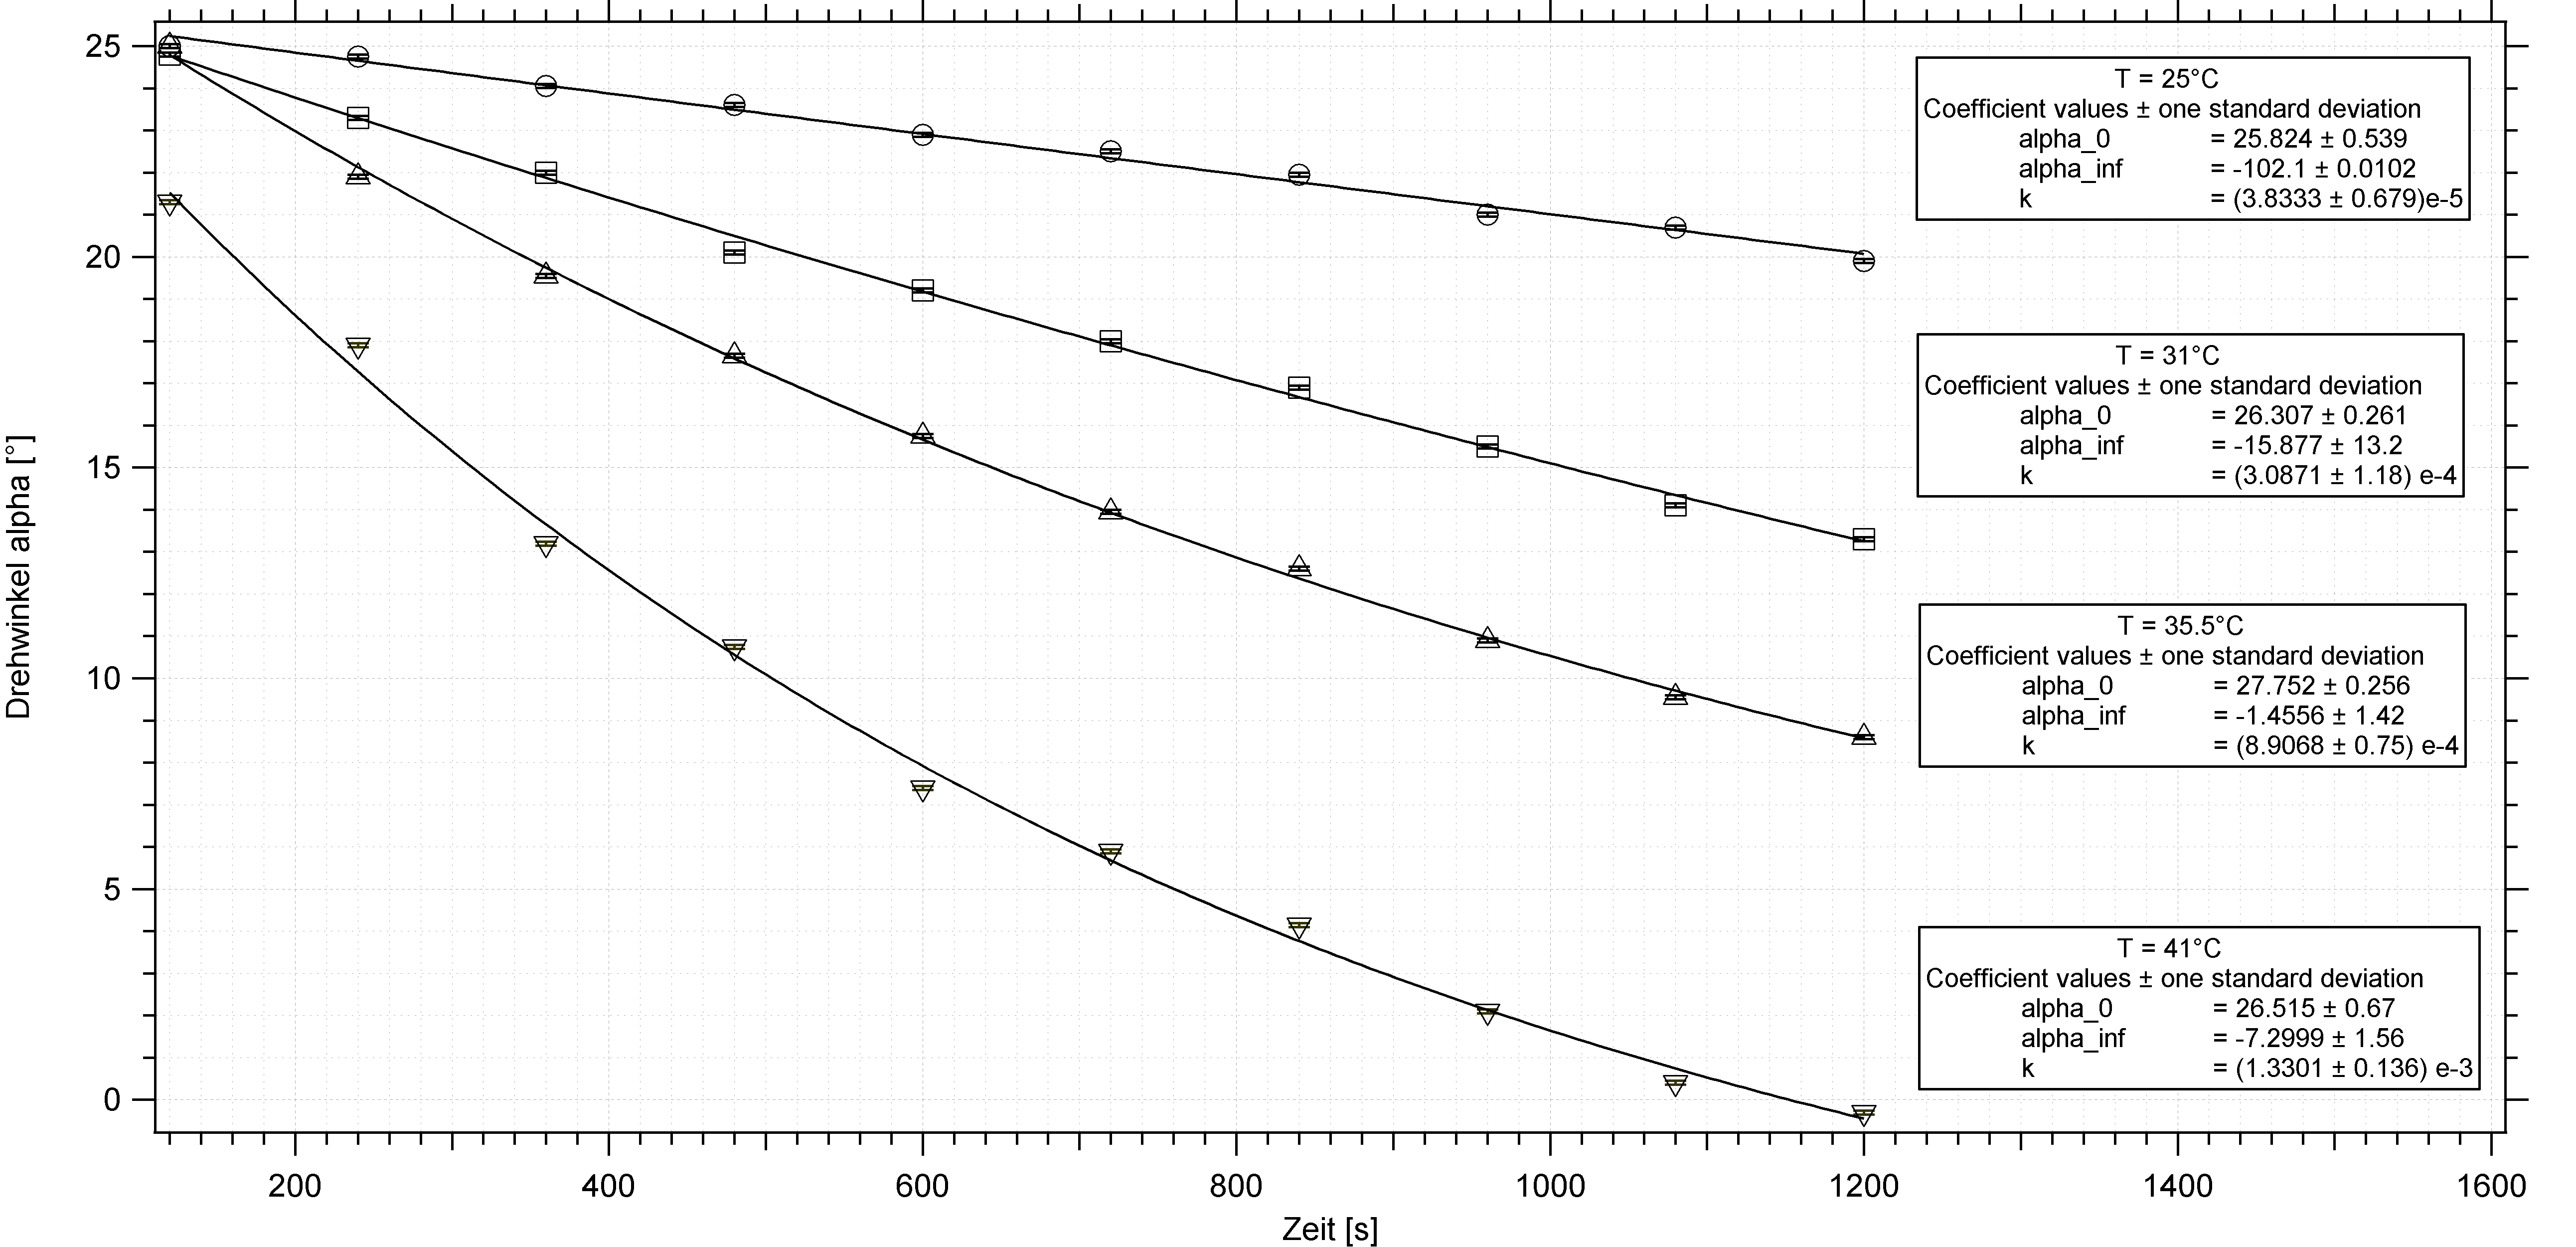
\includegraphics[width=\columnwidth]{Bilder/Graph1.png}
	\end{minipage}
		\caption{Auftragung des optischen Drehwinkels gegen die Zeit bei 25°C, 31°C, 35.5°C, 41°C zur Bestimmung von$\alpha_0$, $\alpha_\infty$ sowie von k bei der Hydrolyse von Saccharose ($25 Gew.\%$) mit $3-N$ HCL. Die Auswertung erfolgte mit Igor Pro 6.37 und einer, vom Assistenten zur Verfügung gestellten, Anpassungsfunktion.}
	\label{at}
\end{figure}
%%%%%%%%%%%%%%%%%%%%%%%

\begin{table}[H]
\centering

 
 
 \caption{Zusammenfassung der Reaktionskonstanten der Anpassung  in Relation zur Temperatur.}
\begin{tabular}{L{0.3\linewidth}L{0.3\linewidth}}
Temperatur [\text{\textdegree}C] & Reaktionskonstante $[\si{s}^{-1}]$ \\
\hline \addlinespace[1ex] 
$25$ & $3.83\cdot 10^{-5}$ \\
$31$ & $3.09\cdot 10^{-4}$ \\
$35.5$ & $8.91\cdot 10^{-4}$ \\
$41$ & $1.33\cdot 10^{-3}$ \\
 \end{tabular}
 \label{tab1}
 \end{table}

Anschießend wurden der Natürliche Logarithmus von $k_T$ gegen $\frac{1}{T}$ gemäß der Arrhenius-Gleichung \ref{eq:logarithmArrhenius} aufgetragen. Durch eine lineare Regression konnten somit $E_a$ und $k_\infty$ bestimmt werden. Dies ist in Abbildung \ref{ln} dargestellt.
\begin{figure}[H]
	\centering	
	\begin{minipage}{1\textwidth}
	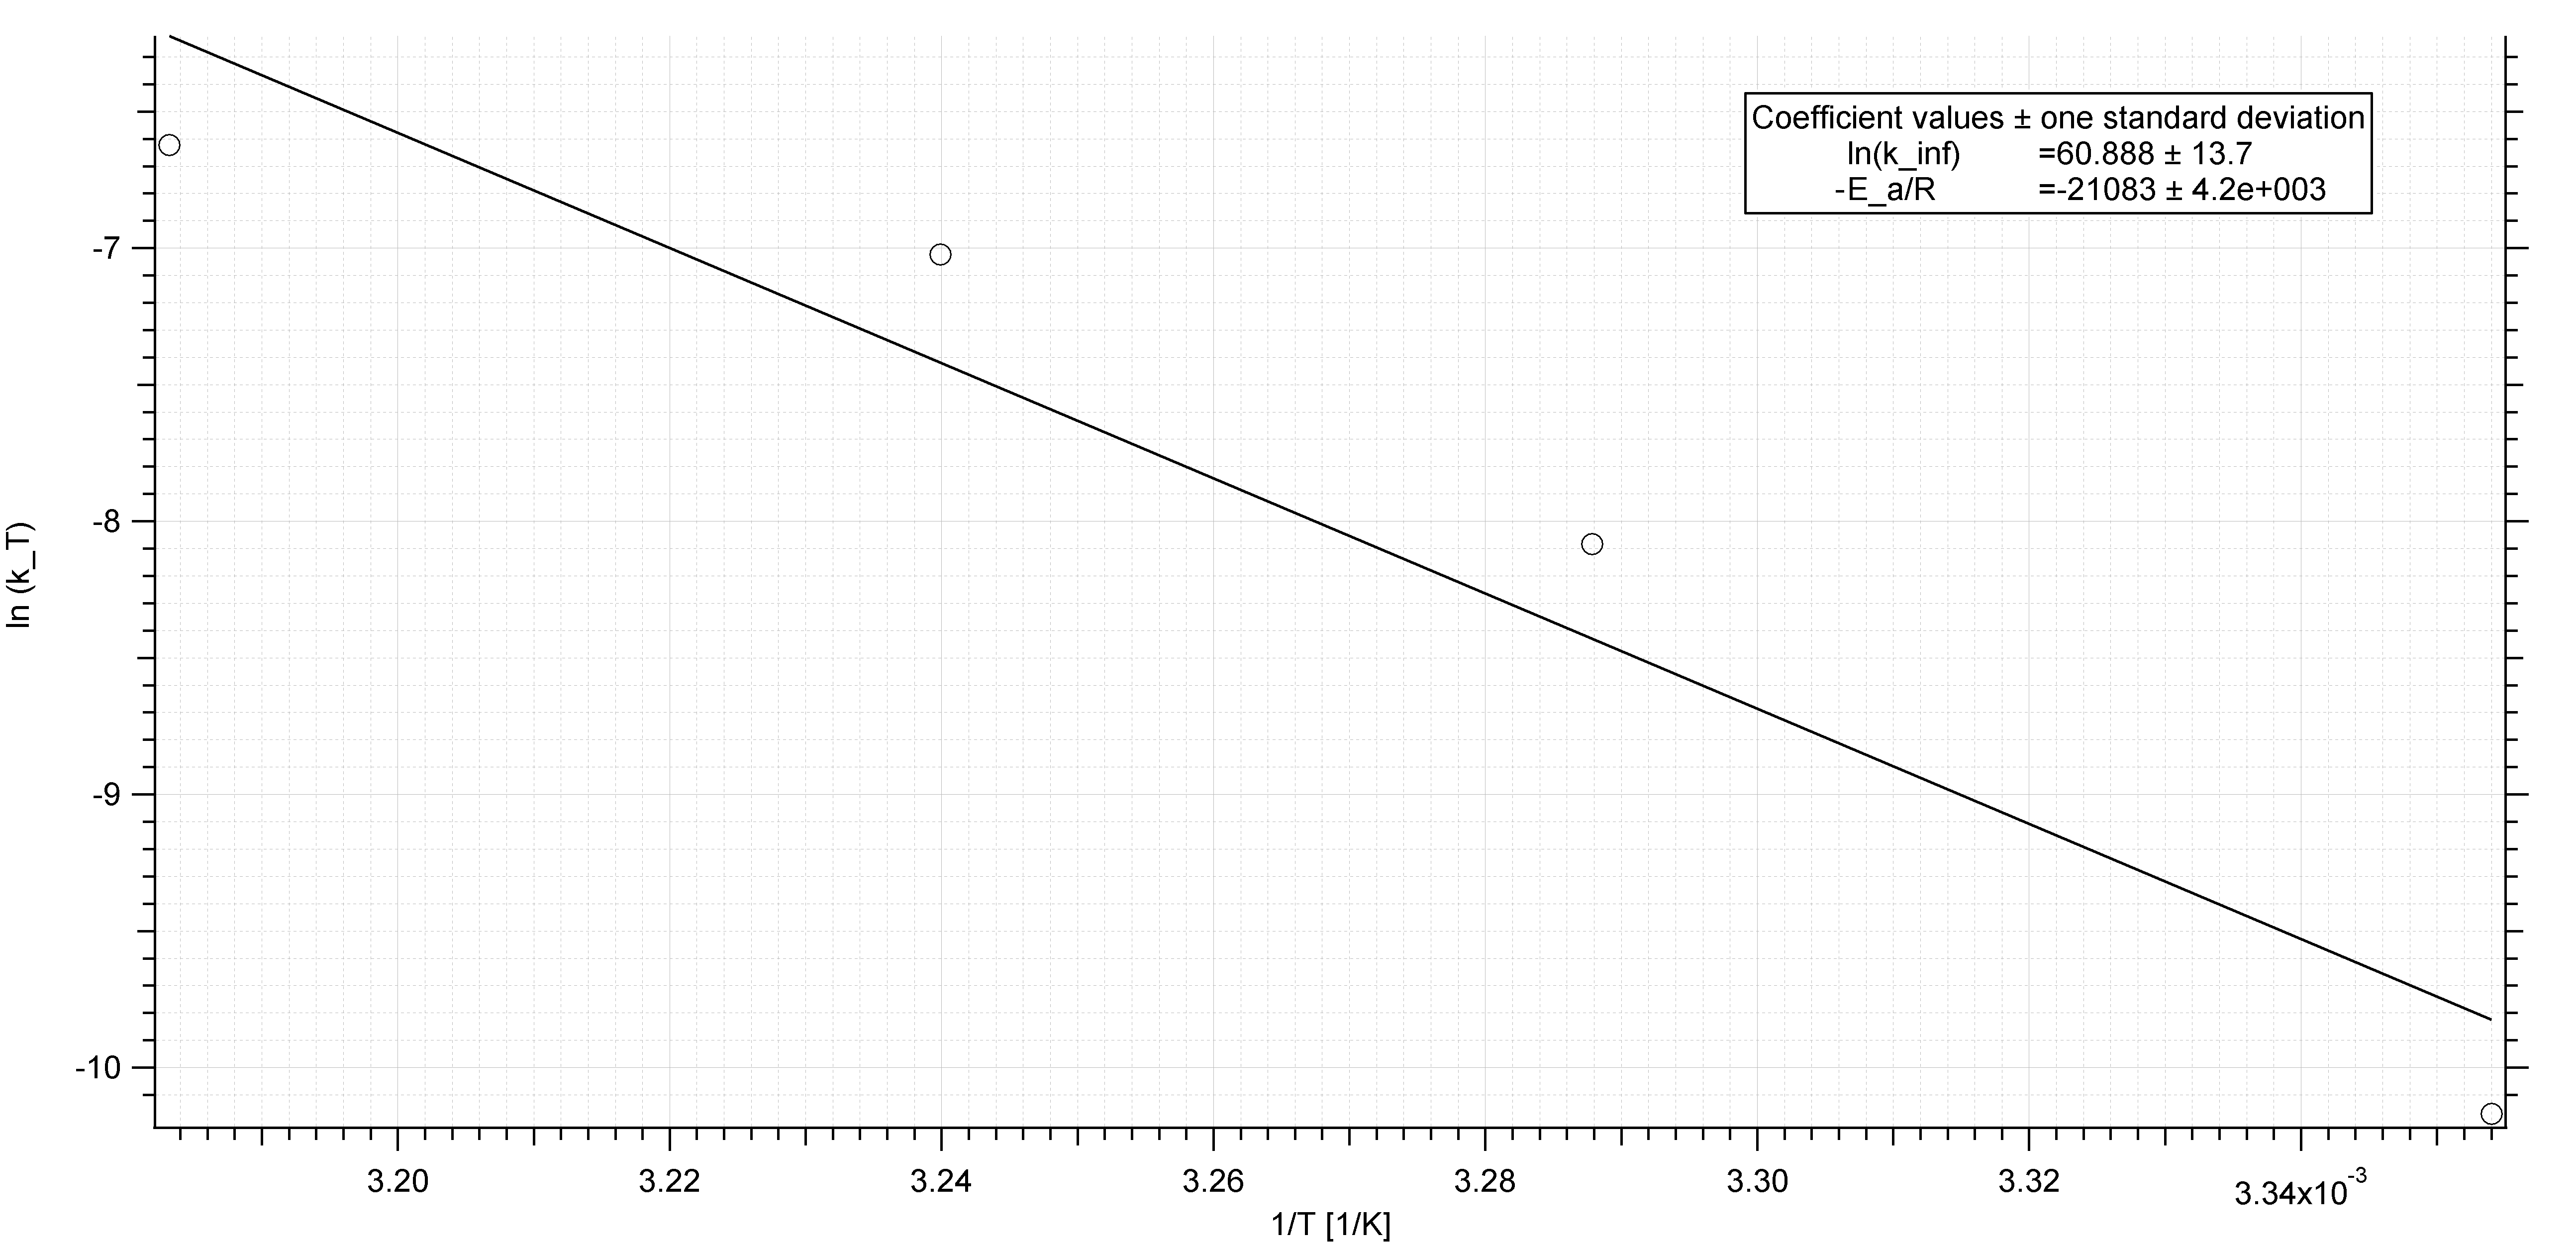
\includegraphics[width=\columnwidth]{Bilder/Graph2.png}
	\end{minipage}	
	\caption{Auftragung von $k_T$ über $\frac{1}{T}$ zur Bestimmung von $E_a$ und $k_\infty$ mittels einer linearen Regression der logarithmierten Arrhenius-Gleichung. Die Auswertung erfolgte mit Igor Pro 6.37}
	\label{ln}
\end{figure}

\begin{table}[H]
\centering
 
 
 \caption{Zusammenfassung der Ergebnisse der lineraren Regression der logarithmierten Arrhenius-Gleichung in Gegenüberstellung zur Literatur.}
\begin{tabular}{L{0.2\linewidth}L{0.2\linewidth}L{0.20\linewidth}R{0.2\linewidth}}
Konstante & Einheit & Messwert & Literatur \cite{saclit}\\
\hline \addlinespace[1ex] 
$ k_\infty$ & $ \frac{1}{s} $ & $ 2.77\cdot 10^{26}$  & \\
\addlinespace[1ex]
$ E_a $ & $ \frac{kJ}{mol} $ & $175 \pm 35$ & $108.4$\\


 \end{tabular}
 \label{tab2}
 \end{table}

Beim Vergleich mit den Literaturwerten in Tabelle \ref{tab2} fällt auf, dass die gemessenen Werte signifikant abweichen. Mögliche Fehlerquellen sind hierbei die Messungenauigkeit bei der Temperatur, der Zeit und des Optischen Drehwinkels. Besonders die Temperatur hat einen großen Einfluss, da geringe Änderungen schon $k$ beeinflussen, was dann durch das potenzieren zu einer sehr großen Abweichung in  $k_\infty$  führt. 

%\end{document}
